% Foliensatz: "AFu-Kurs nach DJ4UF" von DK0TU, Amateurfunkgruppe der TU Berlin
% Lizenz: CC BY-NC-SA 3.0 de (http://creativecommons.org/licenses/by-nc-sa/3.0/de/)
% Autoren: Sebastian Lange <dl7bst@dk0tu.de>, Lars Weiler <dc4lw@darc.de>

\documentclass[aspectratio=169]{beamer}

\usepackage[ngerman]{babel} % deutsche Worttrennung etc.
\usepackage[utf8]{inputenc} % UTF8 Text

\usepackage[super, comma, numbers, square, sort]{natbib}

\usepackage{hyperref}       % Hyperref Package für bessere Referenzen (todo)
\hypersetup{
	colorlinks=false,       %   false: boxed links; true: colored links
    %linkcolor=white,       %   color of internal links (change box color with linkbordercolor)
    citecolor=red,          %   color of links to bibliography
    filecolor=white,        %   color of file links
    urlcolor=blue           %   color of external links
}

\usepackage{multirow}
\usepackage{wasysym}  % Math Symbols like \permil
%\usepackage{colortbl}
%\usepackage{subscript}
%\usepackage{caption}
%\usepackage{setspace}
%\usepackage{xcolor}        % benutze CodeListe

% Footnote
%\usepackage{hanging}
%
%\setbeamertemplate{footnote}{%
%  \hangpara{2em}{1}%
%  \makebox[2em][l]{\insertfootnotemark}\footnotesize\insertfootnotetext\par%
%}


%\usepackage{pgf}
%\usepackage{tikz}
%\usetikzlibrary{arrows,automata}
%\usetikzlibrary{positioning}
%
%\tikzset{
%    state/.style={
%           rectangle,
%           rounded corners,
%           draw=black, very thick,
%           minimum height=2em,
%           minimum width=2pt,
%           inner sep=2pt,
%           text centered,
%           },
%}

%\usepackage{listings}
%\lstset{basicstyle=\small, numberstyle=\tiny, extendedchars=true, numbers=left, numbersep=5pt}
%\lstset{showtabs=false, showspaces=false, showstringspaces=false}
%%\lstset{backgroundcolor=\color{white!75!lightgray}, , frame=single}
%%\lstset{backgroundcolor=\color{white}}
%%\lstset{backgroundcolor=none}
%\lstset{keywordstyle=\color{blue!50!gray},  identifierstyle=\color{black}}
%\lstset{commentstyle=\color{green!50!gray}, stringstyle=\color{red!50!gray}}
%\lstset{language=C, fontadjust=true, tabsize=2, breaklines=true}
%\lstset{backgroundcolor=\color{white!75!lightgray}, caption=\lstname, frame=single}
%\lstset{emphstyle=\color{black}\fbox}
%
%% Keine "Listing:"-Caption
%\captionsetup{labelformat=empty,labelsep=none}
%
%% für mathematische Umgebungen
%\usepackage{amsmath,amsfonts,amssymb}
%
%\lstdefinestyle{Bash}{
%language=Bash,
%frame=single,
%rulecolor=\color{black},
%backgroundcolor=\color{gray!50},
%keywordstyle=\color{black},
%identifierstyle=,
%commentstyle=\color{black},
%stringstyle=\color{magenta!65!white},
%showstringspaces=false,
%basicstyle=\footnotesize\ttfamily\color{black},
%numbers=none,
%breaklines=true,
%captionpos=b
%}

%\usepackage{listings}
%
%\lstdefinestyle{basic}{
%    captionpos=t,%
%    basicstyle=\footnotesize\ttfamily,%
%    numberstyle=\tiny,%
%    numbers=left,%
%    stepnumber=1,%
%    frame=single,%
%    showspaces=false,%
%    showstringspaces=false,%
%    showtabs=false,%
%    %
%    keywordstyle=\color{blue},%
%    identifierstyle=,%
%    commentstyle=\color{gray},%
%    stringstyle=\color{magenta}%
%}



% fließende Boxen haben keinen Abstand
%\fboxsep0mm

% inkludiere Creative Commons Helper
%%%%%%%%%%%%%%%%%%%%%%%%%%%%%%%%%%%%%%%%%%%%%%%%%%%%%%%%%%%%%%%%
%% ccBeamer 0.1, 2007-07-02                                   %%
%% Written by Sebastian Pipping <webmaster@hartwork.org>      %%
%% ---------------------------------------------------------- %%
%% Licensed under Creative Commons Attribution-ShareAlike 3.0 %%
%% http://creativecommons.org/licenses/by-sa/3.0/             %%
%%%%%%%%%%%%%%%%%%%%%%%%%%%%%%%%%%%%%%%%%%%%%%%%%%%%%%%%%%%%%%%%


%% Images
\newcommand{\CcImageBy}[1]{%
	
\includegraphics[scale=#1]{texdata/creative_commons/cc_by_30.pdf}%
}
\newcommand{\CcImageCc}[1]{%
	
\includegraphics[scale=#1]{texdata/creative_commons/cc_cc_30.pdf}%
}
\newcommand{\CcImageDevNations}[1]{%
	
\includegraphics[scale=#1]{texdata/creative_commons/cc_dev_nations_30.pdf}%
}
\newcommand{\CcImageNc}[1]{%
	
\includegraphics[scale=#1]{texdata/creative_commons/cc_nc_30.pdf}%
}
\newcommand{\CcImageNd}[1]{%
	
\includegraphics[scale=#1]{texdata/creative_commons/cc_nd_30.pdf}%
}
\newcommand{\CcImagePd}[1]{%
	
\includegraphics[scale=#1]{texdata/creative_commons/cc_pd_30.pdf}%
}
\newcommand{\CcImageSa}[1]{%
	
\includegraphics[scale=#1]{texdata/creative_commons/cc_sa_30.pdf}%
}
\newcommand{\CcImageSampling}[1]{%
	
\includegraphics[scale=#1]{texdata/creative_commons/cc_sampling_30.pdf}%
}
\newcommand{\CcImageSamplingPlus}[1]{%
	
\includegraphics[scale=#1]{texdata/creative_commons/cc_sampling_plus_30.pdf}%
}


%% Groups
\newcommand{\CcGroupBy}[2]{% zoom, gap
	\CcImageCc{#1}\hspace*{#2}\CcImageBy{#1}%
}
\newcommand{\CcGroupByNc}[2]{% zoom, gap
	\CcImageCc{#1}\hspace*{#2}\CcImageBy{#1}\hspace*{#2}\CcImageNc{#1}%
}
\newcommand{\CcGroupByNcNd}[2]{% zoom, gap
	\CcImageCc{#1}\hspace*{#2}\CcImageBy{#1}\hspace*{#2}\CcImageNc{#1}\hspace*{#2}\CcImageNd{#1}%
}
\newcommand{\CcGroupByNcSa}[2]{% zoom, gap
	\CcImageCc{#1}\hspace*{#2}\CcImageBy{#1}\hspace*{#2}\CcImageNc{#1}\hspace*{#2}\CcImageSa{#1}%
}
\newcommand{\CcGroupByNd}[2]{% zoom, gap
	\CcImageCc{#1}\hspace*{#2}\CcImageBy{#1}\hspace*{#2}\CcImageNd{#1}%
}
\newcommand{\CcGroupBySa}[2]{% zoom, gap
	\CcImageCc{#1}\hspace*{#2}\CcImageBy{#1}\hspace*{#2}\CcImageSa{#1}%
}
\newcommand{\CcGroupDevNations}[2]{% zoom, gap
	\CcImageCc{#1}\hspace*{#2}\CcImageDevNations{#1}%
}
\newcommand{\CcGroupNcSampling}[2]{% zoom, gap
	\CcImageCc{#1}\hspace*{#2}\CcImageNc{#1}\hspace*{#2}\CcImageSampling{#1}%
}
\newcommand{\CcGroupPd}[1]{% zoom
	\CcImagePd{#1}%
}
\newcommand{\CcGroupSampling}[1]{% zoom
	\CcImageSampling{#1}%
}
\newcommand{\CcGroupSamplingPlus}[1]{% zoom
	\CcImageSamplingPlus{#1}%
}


%% Text
\newcommand{\CcLongnameBy}{Attribution}
\newcommand{\CcLongnameByNc}{Attribution-NonCommercial}
\newcommand{\CcLongnameByNcNd}{Attribution-NoDerivs}
\newcommand{\CcLongnameByNcSa}{Attribution-NonCommercial-ShareAlike}
\newcommand{\CcLongnameByNd}{Attribution-NoDerivs}
\newcommand{\CcLongnameBySa}{Attribution-ShareAlike}

\newcommand{\CcNote}[1]{% longname
	This work is licensed under the \textit{Creative Commons #1 3.0 License}.%
}


% generelles Thema auswählen
\usetheme{Goettingen} %Berlin spart ohne Sidebar allerdings angenehm Platz
% AnnArbor | Antibes | Bergen | Berkeley | Berlin | Boadilla | boxes | CambridgeUS | Copenhagen | Darmstadt | default | Dresden | Frankfurt | Goettingen | Hannover | Ilmenau | JuanLesPins | Luebeck | Madrid | Malmoe | Marburg | Montpellier | PaloAlto | Pittsburgh | Rochester | Singapore | Szeged | Warsaw

% Farben wählen
\usecolortheme{beetle}
% beaver | beetle | crane | default | dolphin | dove | fly | lily | orchid | rose | seagull | seahorse | sidebartab | structure | whale | wolverine

% Setze alle Farben auf Grau und Weiß
%\definecolor{craneorange}{RGB}{64,64,64}
%\definecolor{craneblue}{RGB}{255,255,255}

% Schriftart wählen
\usefonttheme{default}
% default | professionalfonts | serif | structurebold | structureitalicserif | structuresmallcapsserif

% Innere Themen(Kopf-, Fuß-, Sidebar usw)
%\useinnertheme{default}
\useinnertheme{circles}
% default | inmargin | rectangles | rounded | circles

% Äußere Themen (Anordnung der inneren, grenzen der Folien etc.)
\useoutertheme{infolines}
% default | infolines | miniframes | shadow | sidebar | smoothbars | smoothtree | split | tree

% Deaktiviere Navigations-Symbole ({} -> leer)
\setbeamertemplate{navigation symbols}{}
%\setbeamertemplate{navigation symbols}{\large \ifnum \insertframenumber <10 0\fi\insertframenumber/\inserttotalframenumber\vspace*{0.2ex}}

% Zeige ein Hintergrundbild
\setbeamertemplate{background canvas}{
        \hspace*{-2.0cm}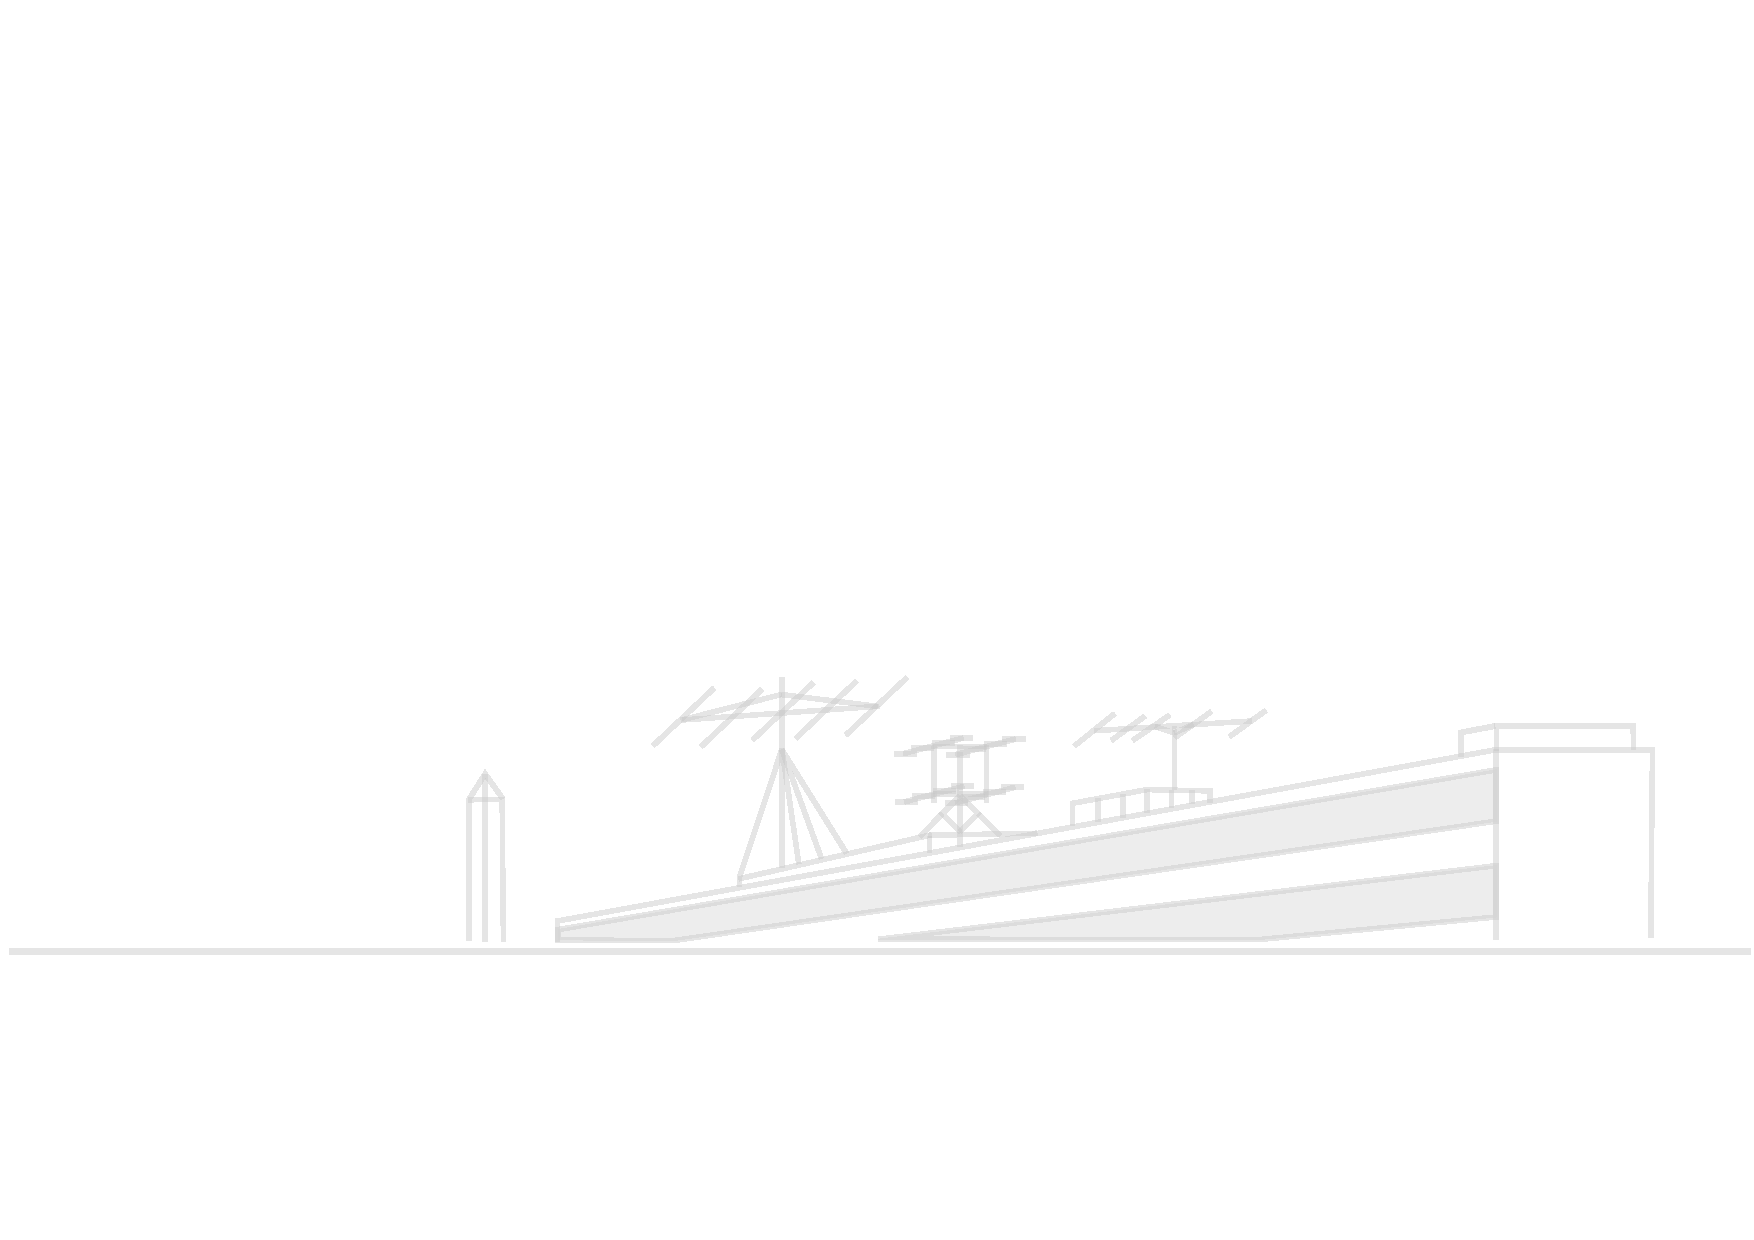
\includegraphics[width=17.8cm]{texdata/dk0tu_rooftop_background.pdf}
}

% Foliennummer einfügen
\setbeamertemplate{footline}[frame number]
%\setbeamertemplate{footline}{}

% Ändere das Zeichen vor jedem item
%\setbeamertemplate{itemize item}{\color{craneorange}$\blacktriangleright$}
%\setbeamertemplate{itemize subitem}{\color{craneorange}$\triangleright$}
%\setbeamertemplate{itemize subsubitem}{\color{craneorange}$\blacktriangleright$}

% Ändert die Blöcke 
\setbeamertemplate{blocks}[rounded][shadow=true]
% default | rounded [shadow=true|false]

%
% Eigene Kommandos
%

% Hack to get natbib and beamer working together. "The beamer user guide suggests
% that only the manual bibliography entry approach is supported"
% on some system it works out of the box, sometimes you need the hack :-(
% so check it --dl7bst
\ifdefined\newblock
    \relax
\else
    \newcommand{\newblock}{}
\fi

% \includedia command to generate png out of a dia file
% NEEDS installed dia and pdflatex option --shell-escape
\newcommand{\includedia}[1]{
    \immediate\write18{/usr/bin/dia #1.dia -e #1_diatmp.png -t png}
}

% RICHIG GROSSER FONT!
\newfont{\bigfont}{cmr10 at 144pt}
\newfont{\smallfont}{cmr10 at 8pt}

% Römische Ziffern
\makeatletter
\newcommand{\rmnum}[1]{\romannumeral #1}
\newcommand{\Rmnum}[1]{\expandafter\@slowromancap\romannumeral #1@}
\makeatother

% Schwarze Überschrift
%\setbeamercolor{frametitle}{fg=black}
%\setbeamercolor{title}{fg=black}

% Item- und Box-Farben
\definecolor{deepBlue}{HTML}{000066}
\setbeamercolor{itemize item}{fg=deepBlue}
\setbeamercolor{itemize subitem}{fg=deepBlue}
\setbeamercolor{description item}{fg=deepBlue}
\setbeamercolor{block title}{fg=deepBlue!100, bg=blue!15}
\setbeamercolor{block body}{fg=black, bg=blue!5}
\setbeamercolor{block title alerted}{fg=deepBlue, bg=red!75}
\setbeamercolor{block body alerted}{fg=black, bg=red!15}
\setbeamercolor*{block title example}{fg=blue!50, bg=blue!10}
\setbeamercolor*{block body example}{fg= blue, bg=blue!5}

%\setbeamercolor{section in head/foot}{parent=palette primary}
%\setbeamercolor{subsection in head/foot}{parent=palette secondary}
%\setbeamercolor{sidebar}{fg=darkblue,bg=yellow!90!orange}
%\setbeamercolor{title in sidebar}{fg=darkblue}
%\setbeamercolor{author in sidebar}{fg=darkblue}
%\setbeamercolor{section in sidebar}{fg=darkblue!10!black}
%\setbeamercolor{subsection in sidebar}{fg=darkblue!50!black}

% Titlepage Infos
\title{AFu-Kurs nach DJ4UF}
\author[DKØTU]{DKØTU\\ \footnotesize{Amateurfunkgruppe der TU Berlin}}
\institute[DKØTU]{\url{http://www.dk0tu.de} }

% PDF-Eigenschaften
\subject{DK0TU-Amateurfunkkurs nach DJ4UF}
\keywords{Amateurfunk Kurs HAM Radio Course CC-BY-NC-SA OpenSource TU Berlin DK0TU}

\subtitle{Technik Klasse A 12: \\
  Modulation und Demodulation \\[2em]}
\date{Stand 15.02.2016}
 \begin{document}

\begin{frame}
    \titlepage
    \vfill
    \begin{center}
        \ccbyncsaeu\\
        {\tiny This work is licensed under the \em{Creative Commons Attribution-NonCommercial-ShareAlike 3.0 License}.}\\[0.5ex]
         \tiny Amateurfunkgruppe der Technische Universität Berlin (AfuTUB), DKØTU
         %\includegraphics[scale=0.5]{img/DK0TU_Logo.pdf}
    \end{center}
\end{frame}


\section{Überblick}

\begin{frame}
  \frametitle{Überblick}

  Wiederholung: Was ist Modulation? \bigskip

  Nennt die Prinzipien von:

  \begin{itemize}
    \item AM
    \item SSB
    \item FM
  \end{itemize}

  \pause

  Diese Lektion setzt viele unterschiedliche Schaltungsbilder ein -- nicht abschrecken lassen!

\end{frame}


\section{AM}

\subsection{Modulation}

\begin{frame}
  \frametitle{AM-Modulation}

  \begin{columns}
    \column{.4\textwidth}
    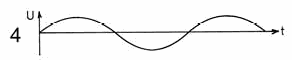
\includegraphics[width=\textwidth,height=.3\textheight,keepaspectratio]{a12/td503d.png}
    \column{.5\textwidth}
    NF-Signal wird gemischt mit einem
  \end{columns}
  \begin{columns}
    \column{.4\textwidth}
    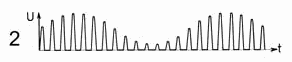
\includegraphics[width=\textwidth,height=.3\textheight,keepaspectratio]{a12/td503b.png}
    \column{.5\textwidth}
    HF-Signal. Beim resultierenden Signal (nicht dargestellt) wird durch
  \end{columns}
  \begin{columns}
    \column{.4\textwidth}
    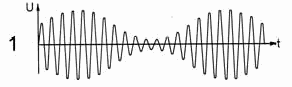
\includegraphics[width=\textwidth,height=.3\textheight,keepaspectratio]{a12/td503a.png}\\
    {\tiny TD503}
    \column{.5\textwidth}
    eine Diode eine Halbwelle entfernt. Mit einer Siebschaltung werden die fehlenden Halbwellen mit gleicher Größe der vorhandenen regeneriert.
  \end{columns}
\end{frame}


\subsubsection{Modulations"-grad}

\begin{frame}
  \frametitle{AM-Modulationsgrad}

  \begin{block}{Modulationsgrad}
    Verhältnis der Amplitude der NF-Schwingung zur Amplitude der unmodulierten Trägerschwingung.\\
    $m = \cfrac{\hat{U}_{mod}}{\hat{U}_T}$
  \end{block}

  \begin{center}
    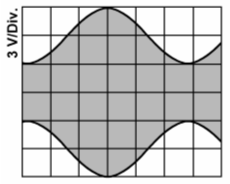
\includegraphics[width=0.5\textwidth,height=.5\textheight,keepaspectratio]{a12/TE111.png}
    {\tiny TE111}
  \end{center}
\end{frame}


\subsubsection{Leistung}

\begin{frame}
  \frametitle{Leistung bei AM}
  \begin{exampleblock}{Beispiel bei 100\% Modulationsgrad}
    100\% Modulationsgrad $\equiv$ Trägerspannung und Modulationsspannung gleich\\[.5em]
    z.B. Gesamtspannung 10V $\Rightarrow$ 5V Träger + 2 Mal 2,5V Seitenfrequenzen\\[.5em]
    Bei einem Widerstand von 50$\Omega$ ergibt sich für die Leistung $P = \frac{U^2}{R}$\\[.5em]
    \begin{align*}
      \text{Träger: } & P       &= \frac{5^2V^2}{50\Omega}   = 0,5W    \\
      \text{Seiten: } & P_{SSB} &= \frac{2,5^2V^2}{50\Omega} = 0,125W \\
      \text{Gesamt: } & P_{ges} &= 0,5W + 2 \cdot 0,125W           = 0,75W  \\
    \end{align*}
    In 1/6 der Gesamtleistung liegt die Information!
  \end{exampleblock}
\end{frame}


\subsection{Demodulation}

\begin{frame}
  \frametitle{AM-Demodulation}

  \begin{columns}
    \column{.5\textwidth}
    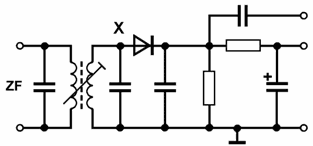
\includegraphics[width=\textwidth,height=\textheight,keepaspectratio]{a12/td503.png}\\
    {\tiny TD501}
    \column{.45\textwidth}
    \textbf{Hüllkurvendemodulator}\\[.5em]
    Bestehend aus Gleichrichter, Diode, Ladekondensator, Entladungswiderstand und Koppelkondensator
  \end{columns}
\end{frame}

\begin{frame}
  \begin{tabular}{l||p{.8\textwidth}}\hline
    \textbf{TD503} & \textbf{Am ZF-Eingang liegt ein sinusförmig moduliertes AM-Signal. Bei dieser Schaltung zeigt der mit ``X'' bezeichnete Punkt das nebenstehende}
    \begin{tabular}[c]{lr}
      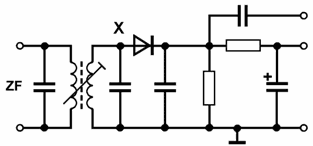
\includegraphics[width=.4\textwidth,height=.4\textheight,keepaspectratio]{a12/td503.png} &
      \parbox[c]{.3\textwidth}{
      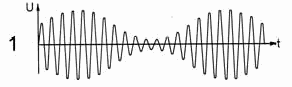
\includegraphics[width=.3\textwidth]{a12/td503a.png}\\
      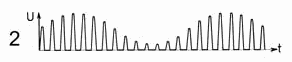
\includegraphics[width=.3\textwidth]{a12/td503b.png}\\
      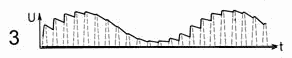
\includegraphics[width=.3\textwidth]{a12/td503c.png}\\
      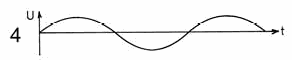
\includegraphics[width=.3\textwidth]{a12/td503d.png}\\
      }\\
    \end{tabular}\\ \hline\hline
    A \only<2>\checkmark & Signal 1. \\ \hline
    B & Signal 2. \\ \hline
    C & Signal 3. \\ \hline
    D & Signal 4. \\ \hline
  \end{tabular}
\end{frame}

\begin{frame}
  \begin{tabular}{l||p{.8\textwidth}}\hline
    \textbf{TD504} & \textbf{Am ZF-Eingang liegt ein sinusförmig moduliertes AM-Signal. Bei dieser Schaltung zeigt der mit ``X'' bezeichnete Punkt das nebenstehende}
    \begin{tabular}[c]{lr}
      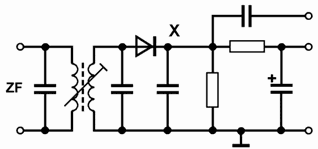
\includegraphics[width=.4\textwidth,height=.4\textheight,keepaspectratio]{a12/td504.png} &
      \parbox[c]{.3\textwidth}{
      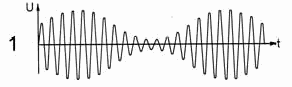
\includegraphics[width=.3\textwidth]{a12/td503a.png}\\
      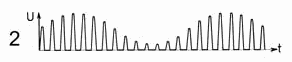
\includegraphics[width=.3\textwidth]{a12/td503b.png}\\
      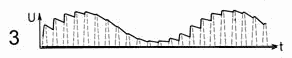
\includegraphics[width=.3\textwidth]{a12/td503c.png}\\
      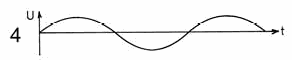
\includegraphics[width=.3\textwidth]{a12/td503d.png}\\
      }\\
    \end{tabular}\\ \hline\hline
    A & Signal 1. \\ \hline
    B & Signal 2. \\ \hline
    C \only<2>\checkmark & Signal 3. \\ \hline
    D & Signal 4. \\ \hline
  \end{tabular}
\end{frame}

\begin{frame}
  \begin{tabular}{l||p{.8\textwidth}}\hline
    \textbf{TF317} & \textbf{Bei dieser Schaltung handelt es sich um einen}
    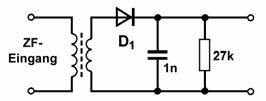
\includegraphics[width=.6\textwidth,height=.5\textheight,keepaspectratio]{a12/tf317.png} \\ \hline\hline
    A & FM-Diskriminator. \\ \hline
    B \only<2>\checkmark & AM-Detektor. \\ \hline
    C & ZF-Modulator. \\ \hline
    D & AGC-Gleichrichter. \\ \hline
  \end{tabular}
\end{frame}


%\subsubsection{Audion}


\subsection{Träger"-unter"-drückung}

\begin{frame}
  \frametitle{Trägerunterdrückung}

  \begin{exampleblock}{Rückblick auf die Mischung}
    Welche Frequenzen entstehen bei der Mischung von 2kHz mit 7,1MHz?\\[1.5em]

    \pause
    $f_1 = 7,098 MHz$ und $f_2 = 7,102 MHz$\\[1.5em]
    $\Rightarrow$ Die Seitenfrequenzen liegen bereits im HF-Bereich und können von einer Antenne abgestrahlt werden!
  \end{exampleblock}
  \pause
  \begin{itemize}
    \item die Leistung des Trägers kann in die Seitenbänder gesteckt werden
    \item der Träger muss am Empfänger für die Demodulation wieder hinzugemischt werden
  \end{itemize}
\end{frame}

\begin{frame}
  \frametitle{Ringmodulator}
  \begin{columns}
    \column{.5\textwidth}
    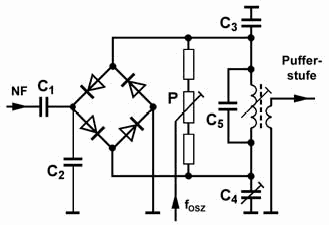
\includegraphics[width=\textwidth,height=.8\textheight,keepaspectratio]{a12/td513.png}\\
    {\tiny TD513}
    \column{.45\textwidth}
    \emph{Das ist keine Gleichrichterschaltung! Die Dioden sind anders angeordnet.}\\[1.5em]
    Je nach Polarität des NF-Signals wird ein anderes Dioden-Pärchen leitend. Bei Polaritätswechsel ergibt sich eine Phasendrehung des modulierten Signals.\\[2.5em]
    {\small Erklärung ist umfangreicher; es gibt nur dieses eine Bild in der Prüfung $\rightarrow$ einfach merken, dass es sich um einen \emph{Modulator zur Erzeugung von AM-Signalen mit unterdrücktem Träger} handelt}
  \end{columns}

\end{frame}


\section{SSB}

\subsection{Modulation}

\begin{frame}
  \frametitle{SSB}

  \begin{itemize}
    \item in beiden Seitenbändern steckt dieselbe Information
    \item durch einen Filter eines der beiden Seitenbänder weglassen
    \item historisch bedingt im Amateurfunk
      \begin{description}
        \item[$f < 10MHz$] Unteres Seitenband (Lower Sideband \textbf{LSB})
        \item[$f > 10MHz$] Oberes Seitenband (Upper Sideband \textbf{USB})
      \end{description}
    \item 5/6 der Leistung von AM kann ohne Informationsverlust in ein Seitenband gesteckt werden
    \item weniger als die Hälfte der Bandbreite von AM
  \end{itemize}
\end{frame}

\begin{frame}
  \begin{tabular}{l||p{.8\textwidth}}\hline
    \textbf{TG213} & \textbf{Wie wird ein SSB-Signal erzeugt?}\\ \hline\hline
    A & Im Balancemodulator wird ein Zweiseitenband-Signal erzeugt. Ein auf die Trägerfrequenz abgestimmter Saugkreis filtert den Träger aus.\\ \hline
    B & Im Balancemodulator wird ein Zweiseitenband-Signal erzeugt. Ein auf die Trägerfrequenz abgestimmter Sperrkreis filtert den Träger aus.\\ \hline
    C \only<2>\checkmark & Im Balancemodulator wird ein Zweiseitenband-Signal erzeugt. Das Seitenbandfilter selektiert ein Seitenband heraus.\\ \hline
    D & Im Balancemodulator wird ein Zweiseitenband-Signal erzeugt. In einem Frequenzteiler wird ein Seitenband abgespalten.\\ \hline
  \end{tabular}
\end{frame}

\begin{frame}
  \begin{tabular}{l||p{.8\textwidth}}\hline
    \textbf{TG214} & \textbf{Für die Erzeugung eines SSB-Signals wird ein Gegentaktmodulator verwendet. Das zur Unterdrückung eines Seitenbandes nachgeschaltete Filter sollte über}\\ \hline\hline
    A \only<2>\checkmark & 2,4 kHz Bandbreite verfügen.\\ \hline
    B & 800 Hz Bandbreite verfügen.\\ \hline
    C & 455 kHz Bandbreite verfügen.\\ \hline
    D & 10,7 MHz Bandbreite verfügen.\\ \hline
  \end{tabular}
\end{frame}


\subsection{Demoduluation}

\begin{frame}
  \frametitle{SSB-Demodulation}

  \begin{itemize}
    \item Zufügen des Trägers, beispielsweise mit einem BFO (beat frequency oscillator)
    \item auch das zweite Seitenband wird damit wiederhergestellt
    \item Ergebnis ist ein normales AM-Signal
    \item ab hier kann ein AM-Demodulator eingesetzt werden
  \end{itemize}
\end{frame}

\begin{frame}
  \begin{tabular}{l||p{.8\textwidth}}\hline
    \textbf{TF418} & \textbf{Ein Empfänger arbeitet mit einer End-ZF von 455 kHz. Welche BFO-Frequenz wäre beim CW-Empfang geeignet?} \\ \hline\hline
    A & 455 kHz.\\ \hline
    B & 465,7 kHz. \\ \hline
    C \only<2>\checkmark & 455,8 kHz. \\ \hline
    D & 10,7 MHz. \\ \hline
  \end{tabular}
\end{frame}


\subsubsection{Produktdetektor}

\begin{frame}
  \begin{tabular}{l||p{.8\textwidth}}\hline
    \textbf{TD511} & \textbf{Bei dieser Schaltung handelt es sich um einen}
    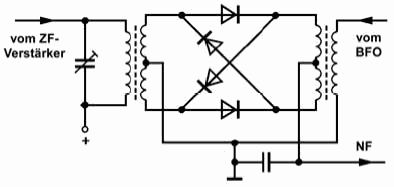
\includegraphics[width=.8\textwidth,height=.5\textheight,keepaspectratio]{a12/td511.png} \\ \hline\hline
    A & Flankendemudolator zur Demodulation von FM-Signalen. \\ \hline
    B & Diskriminator zur Demodulation von FM-Signalen. \\ \hline
    C & Hüllkurvendemodulator zur Demodulation von AM-Signalen. \\ \hline
    D \only<2>\checkmark & Produktdetektor zur Demodulation ven SSB-Signalen. \\ \hline
  \end{tabular}
\end{frame}

\begin{frame}
  \frametitle{Produktdetektor}
  \begin{columns}
    \column{.5\textwidth}
    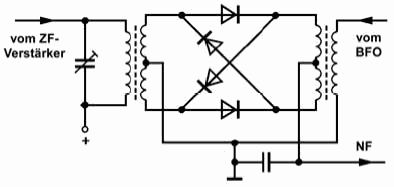
\includegraphics[width=\textwidth,height=.85\textheight,keepaspectratio]{a12/td511.png}\\
    {\tiny TD511}
    \column{.45\textwidth}
    \begin{itemize}
      \item anderer Demodulator anstatt AM-Hüllkurvendemodulator
      \item Ringmodulator (ordne die Dioden anders an, dann wird es deutlich)
      \item jeweils an den Mittenanzapfungen von SSB-Signal und BFO wird das NF-Signal abgenommen
    \end{itemize}
    {\small Auch hier ist die Erklärung wieder umfangreich $\rightarrow$ einfach das Bild und den Begriff \emph{Produktdetektor} merken.}
  \end{columns}
\end{frame}


\section{FM}

\subsection{Modulation}

\begin{frame}
  \frametitle{FM-Modulation}

  \begin{columns}
    \column{.5\textwidth}
    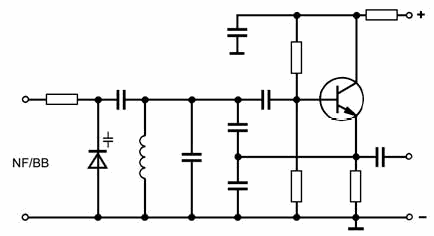
\includegraphics[width=\textwidth,height=.85\textheight,keepaspectratio]{a12/td514.png}\\
    {\tiny TD514}
    \column{.45\textwidth}
    \begin{itemize}
      \item Kapazitätsdiode parallel zum Oszillator geschaltet
      \item bei Amplitudenänderung der NF ändert sich die Sperrspannung des Varicaps
      \item dieses ändert die Frequenz des Oszillators
      \item die Amplitude des Oszillators bleibt gleich
      \item Empfindlichkeit wird in kHz/V angegeben
    \end{itemize}
  \end{columns}
\end{frame}

\begin{frame}
  \begin{tabular}{l||p{.8\textwidth}}\hline
    \textbf{TD514} & \textbf{Bei dieser Schaltung handelt es sich um einen Modulator zur Erzeugung von}
    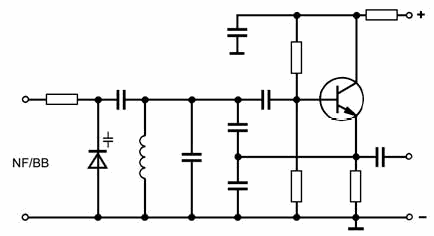
\includegraphics[width=.7\textwidth,height=.85\textheight,keepaspectratio]{a12/td514.png}\\ \hline\hline
    A & phasenmodulierten Signalen. \\ \hline
    B \only<2>\checkmark & frequenzmodulierten Signalen. \\ \hline
    C & AM-Signalen mit unterdrücktem Träger. \\ \hline
    D & AM-Signalen. \\ \hline
  \end{tabular}
\end{frame}

\begin{frame}
  \begin{tabular}{l||p{.8\textwidth}}\hline
    \textbf{TE208} & \textbf{Die Änderung der Kapazität einer über einen Quarzoszillator geschalteten Varicap-Diode stellt eine Möglichkeit dar} \\ \hline\hline
    A \only<2>\checkmark & Frequenzmodulation zu erzeugen. \\ \hline
    B & Zweiseitenbandmodulation zu erzeugen. \\ \hline
    C & CW-Signale zu erzeugen. \\ \hline
    D & Amplitudenmodulation zu erzeugen. \\ \hline
  \end{tabular}
\end{frame}

\begin{frame}
  \begin{tabular}{l||p{.8\textwidth}}\hline
    \textbf{TE216} & \textbf{Wie wird die Empfindlichkeit eines FM-Modulators angegeben?} \\ \hline\hline
    A & in Rad/s \\ \hline
    B & Als Modulationsindex \\ \hline
    C & Als Hub. \\ \hline
    D \only<2>\checkmark & In kHz/V \\ \hline
  \end{tabular}
\end{frame}

\begin{frame}
  \begin{tabular}{l||p{.8\textwidth}}\hline
    \textbf{TG301} & \textbf{Was kann man bezüglich der Ausgangsleistung eines FM-Senders in Abhängigkeit von der Modulation aussagen?}\\ \hline\hline
    A & Sie reduziert sich um 50\%, wenn der Sender moduliert wird. \\ \hline
    B & Sie variiert mit der Modulationsleistung, wenn der Sender moduliert wird. \\ \hline
    C \only<2>\checkmark & Sie ist unabhängig von der Modulation. \\ \hline
    D & Sie geht gegen Null, wenn der Sender nicht moduliert wird. \\ \hline
  \end{tabular}
\end{frame}

\begin{frame}
  \begin{tabular}{l||p{.8\textwidth}}\hline
    \textbf{TG212} &
    \begin{tabular}[c]{lr}
      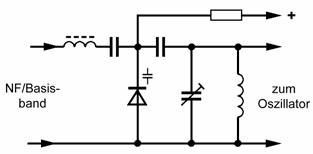
\includegraphics[width=.4\textwidth,height=.5\textheight,keepaspectratio]{a12/tg212.png} &
      \parbox[c]{.4\textwidth}{\textbf{Dieser Schaltungsauszug ist Teil eines Senders.  Welche Funktion hat die Diode?}} \\
    \end{tabular} \\ \hline\hline
    A \only<2>\checkmark & Sie beeinflussst die Resonanzfrequenz des Schwingkreises in Abhängigkeit von den Frequenzen im Basisband und moduliert so die Oszillatorfrequenz. \\ \hline
    B & Sie richtet das Eingangssignal gleich und erzeugt so die Betriebsspannung für den Oszillator, um diesen von der Stromversorgung der anderen Stufen zu entkoppeln. \\ \hline
    C & Sie begrenzt die Amplituden des Eingangssignals und vermeidet so die Übersteuerung der Oszillatorstufe. \\ \hline
    D & Sie dient zur Erzeugung von Amplitudenmodulation und zur Abstimmung der Oszillatorfrequenz. \\ \hline
  \end{tabular}
\end{frame}


\subsubsection{Preemphasis}

\begin{frame}
  \begin{tabular}{l||p{.8\textwidth}}\hline
    \textbf{TB804} & \textbf{Warum wird bei FM senderseitig eine Preemphasis eingesetzt?} \\ \hline\hline
    A & Um das FM Kanalraster von 25 kHz auf 12,5 kHz durch Reduzierung der Bandbreite zu ermöglichen. \\ \hline
    B & Um das breibandige FM-Signal durch Anheben der Amplituden der höheren Modulationsfrequenzen auf Schmalband FM zu reduzieren. \\ \hline
    C & Um die Ausgangsleistung durch Verdichtung des Spektrums der Modulationsfrequenzen zu erhöhen. \\ \hline
    D \only<2>\checkmark & Um das Signal/Rausch-Verhältnis durch Anheben der Amplituden der höheren Modulationsfrequenzen zu verbessern. \\ \hline
  \end{tabular}
\end{frame}


\subsection{Demodulation}

\begin{frame}
  \frametitle{FM-Demodulation}

  \begin{columns}
    \column{.5\textwidth}
    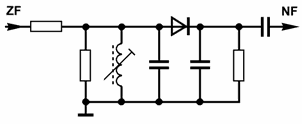
\includegraphics[width=\textwidth,height=.85\textheight,keepaspectratio]{a12/td505.png}\\
    {\tiny TD505}
    \column{.45\textwidth}
    \begin{itemize}
      \item die meisten FM-Demodulatoren wandeln FM erst in AM oder PM um
      \item Fachbezeichnung: \emph{Diskriminator}, hier ein \textbf{Flanken-Diskriminator}
      \item Schwingkreis liefert bei Resonanzfrequenz die größte Spannung
      \item bei Frequenzen knapp daneben wird die Spannung geringer
      \item Ergebnis ist eine AM-Hüllkurve
      \item anschließend Einweggleichrichter
    \end{itemize}
  \end{columns}
\end{frame}

\begin{frame}
  \begin{tabular}{l||p{.8\textwidth}}\hline
    \textbf{TD506} & \textbf{Bei dieser Schaltung handelt es sich um einen}
    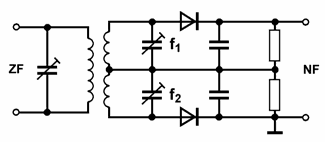
\includegraphics[width=.6\textwidth,height=.4\textheight,keepaspectratio]{a12/td506.png}\\ \hline\hline
    A \only<2>\checkmark & Gegentakt-Flanken-Diskriminator zur Demodulation von FM-Signalen. \\ \hline
    B & Ratiodetektor zur Demodulation von FM-Signalen. \\ \hline
    C & Hüllkurvenmodulator zur Demodulation von AM-Signalen. \\ \hline
    D & Produktdetektor zur Demodulation von SSB-Signalen. \\ \hline
  \end{tabular}
\end{frame}

\begin{frame}
  \begin{columns}
    \column{.5\textwidth}
    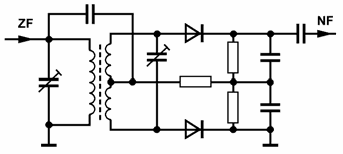
\includegraphics[width=\textwidth,height=.85\textheight,keepaspectratio]{a12/td507.png}\\
    {\tiny TD507}
    \column{.45\textwidth}
    \begin{itemize}
      \item \textbf{Phasendiskriminator}
      \item Wandelt über den Koppelkondensator in Phasenmodulation um
    \end{itemize}
    {\small Diese Schaltung kommt nur ein Mal vor $\rightarrow$ \emph{Kondensator} und \emph{Phasendiskriminator} merken}
  \end{columns}
\end{frame}

\begin{frame}
  \begin{columns}
    \column{.5\textwidth}
    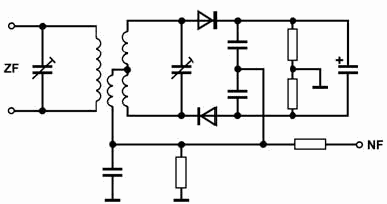
\includegraphics[width=\textwidth,height=.85\textheight,keepaspectratio]{a12/td508.png}\\
    {\tiny TD508}
    \column{.45\textwidth}
    \begin{itemize}
      \item \textbf{Verhältnisdiskriminator} oder \textbf{Ratiodetektor}
      \item ähnlich wie Phasendiskriminator, jedoch mit induktiver Einkopplung
      \item antisymmetrische Dioden
    \end{itemize}
    {\small Diese Schaltung kommt nur ein Mal vor $\rightarrow$ \emph{Dioden} und \emph{Ratiodetektor} merken}
  \end{columns}
\end{frame}

\begin{frame}
  \begin{columns}
    \column{.5\textwidth}
    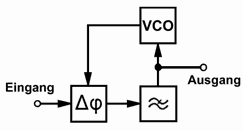
\includegraphics[width=\textwidth,height=.85\textheight,keepaspectratio]{a12/td509.png}\\
    {\tiny TD509}
    \column{.45\textwidth}
    \begin{itemize}
      \item \textbf{PLL-FM-Demodulator}
      \item Demodulation mittels einer PLL (phase locked loop)
      \item VCO ist auf dem FM-Signal eingestellt
      \item ändert sich die HF, wird über den Komparator verglichen
      \item die Änderung soll durch Spannungsänderung nachgeregelt werden
      \item $\Delta V$ entspricht der NF
      \item mehr zu PLL in Lektion A13
    \end{itemize}
    {\small Diese Schaltung kommt nur ein Mal vor $\rightarrow$ \emph{PLL} merken}
  \end{columns}
\end{frame}

\begin{frame}
  \begin{tabular}{l||p{.8\textwidth}}\hline
    \textbf{TD510} & \textbf{Bei dieser Schaltung handelt es sich um einen}
    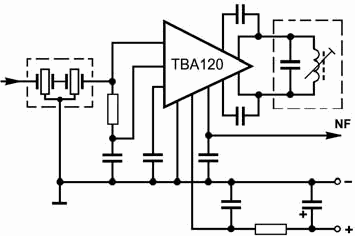
\includegraphics[width=.7\textwidth,height=.5\textheight,keepaspectratio]{a12/td510.png} \\ \hline\hline
    A \only<2>\checkmark & Begrenzerverstärker mit FM-Diskriminator. \\ \hline
    B & Produktdetektor zu Demodulation von SSB-Signalen. \\ \hline
    C & Modulator zur Erzeugung von SSB-Signalen. \\ \hline
    D & Modulator zur Erzeugung von FM-Signalen. \\ \hline
  \end{tabular}

  \only<2>{\vspace{1.5em}ZF-Verstärker mit Quarzfilter, Begrenzer und FM-Demodulator. Einfach merken\ldots}
\end{frame}

\renewcommand{\refname}{Referenzen}

\hypertarget{refs}{}
\textcolor{white}{} \\ %\vspace{} geht nicht
\Large Referenzen/Links
\footnotesize

\begin{thebibliography}{}
  \bibitem{darc}  DARC Online-Lehrgang Lektion A12:
    \url{https://www.darc.de/der-club/referate/ajw/lehrgang-ta/a12/}
  \bibitem{bna}   Fragenkatalog Bundesnetzagentur Technik Klasse A:\\
    \url{https://www.bundesnetzagentur.de/SharedDocs/Downloads/DE/Sachgebiete/Telekommunikation/Unternehmen_Institutionen/Frequenzen/Amateurfunk/Fragenkatalog/TechnikFragenkatalogKlasseAf252rId9014pdf.pdf?__blob=publicationFile&v=3}
\end{thebibliography}

% Hier könnte noch eine Kontaktfolie stehen

\end{document}

